\chapter{Differenziabilità}
\begin{defi}
  Sia $f(x,y)$ definita in D e $P_0(x_0,y_0)\in D$. In $P_0, z=f(x_0,y_0)$, incremento la $x_0$
  di un h e la $y_0$ di un k.\\
  Così passo da $P_0(x_0,y_0)$ a $P(x_0+h,y_0+k)$. La funzione avrà avuto un certo incremento
  \begin{equation*}
    f(x+h,y_0,y_0+k)-f(x_0,y_0)
  \end{equation*}
  Si definisce {\color{red}differenziale} in $P_0(x_0,y_0)$ se
  $\exists A,B \in R: f(x_0+h,y_0+k)-f(x_o,y_0)=Ah+Bk+o(\sqrt{h^2+k^2})$, cioè se esistono
  due costanti reali A e B per cui l'increm,ento di $f(x,y)$ che si ha passando da $P_0$ a $P$
  si può riscrivere come somma di una parte lineare $Ah+Bk$ e di un infinitesimo di ordine
  superiore a $\sqrt{h^2+k^2}$ (\underline{distanza di $P_0$ da $P$}).\\
  Se $f(x,y)$ ammette derivate prime parziali le due costanti A e B sono:
  \begin{equation*}
    \begin{cases}
      A=fx(x_0,y_0)\\
      B=fy(x_0,y_0)
    \end{cases}
  \end{equation*}
  e il differenziale diventa
  \begin{equation}
    f(x_0+h,y_0+k) - f(x_0,y_0)=fx(x_0,y_0)h+fy(x_0,y_0)k+o(\sqrt{h^2+k^2})
  \end{equation}
\end{defi}
\begin{esempio}
  verificare che $z=xy$ è differenziale $\forall (x_0;y_0)\in R^2$, se z è differenziale\\
  $\to f(x_0+h,y_0+k) - f(x_0,y_0)=fx(x_0,y_0)h+fy(x_0,y_0)k+o(\sqrt{h^2+k^2})$ dove
  \begin{equation*}
    \begin{cases}
      A=fx(x_0,y_0)\\
      B=fy(x_0,y_0)
    \end{cases}
  \end{equation*}
  se z è derivabile in ($x_0,y_0$).
  \begin{equation*}
    f(x_0+h,y_0+k) =\underbrace{(x_0+h)(y_0+k)}_{\text{\shortstack{Sostituisco}}}=x_0y_0+x_0k+y_0h+hk
  \end{equation*}
  \begin{multicols}{3}
    $f_x=y\text{ }fx(x_0,y_0)=y_0$\\
    $f$ è derivabile in $(x_0,y_0)$\\
    $f_y=x$\\
    $A=y_0$\\
    $f_y(x_0,y_0)=x_0$\\
    $D=x_0$
  \end{multicols}
  \begin{equation*}
    \begin{matrix}
      f(x_0+h,y_0+k) - f(x_0,y_0)=Ah+Bk+o(\sqrt{h^2+k^2})\\
      \not{x_0y_0}+\not{x_0k}+hk-\not{x_0y_0}=\not{y_0h}+\not{x_0k}+o(\sqrt{h^2+k^2})\\
      hk=o(\sqrt{h^2+k^2})
    \end{matrix}
  \end{equation*}
  detto quindi dimostrare che $\lim\limits_{h\to 0 k\to 0}\frac{hk}{\sqrt{h^2+k^2}}=0$
  e poi passo alle coordinate polari:
  \begin{equation*}
    \begin{matrix}
      h=\rho \cos \theta\\
      k=\rho \sin \theta & \lim\limits_{\rho\to 0} \frac{\not{e} \cos\theta* \not{e} sin\theta}{\not{e}^2}& z=xy \text{ defferenziale } \forall (x_0,y_0)\in R^2\\
      e^2=h^2+k^2\\
      h\to0,k\to 0,\rho \to 0\\
    \end{matrix}
  \end{equation*}  
\end{esempio}
\subsection{Tutte le funzioni differenziali sono continue}
Sia $f(x,y)$ differenziabile $(x_0,y_0)$, allora $f(x,y)$ è continua in $(x_0,y_0)$
\begin{multicols}{2}
  \paragraph{Ip:}
  \begin{equation*}
    f(x,y) \text{ differenziabile in } (x_0,y_0)
  \end{equation*}
  \paragraph{Th:}
  \begin{equation*}
    f(x,y) \text{ è continua in } (x_0,y_0)
  \end{equation*}
\end{multicols}
\begin{proof}
  Poiché $f(x,y)$ è differenziabile in ($x_0,y_0$) vale la relazione
  \begin{equation*}
    f(x_0+h,y_0+k) - f(x_0,y_0)=Ah+Bk+o(\sqrt{h^2+k^2})
  \end{equation*}
  Se $f(x_0,y_0)$ è continua in $(x_0,y_0)$
  \begin{equation*}
    \lim_{h\to 0\text{ } k\to 0}f(x_0+h,y_0+k) - f(x_0,y_0)=0
  \end{equation*}
  Calcolo il limite a destra per $h\to 0$ $k\to 0$
  \begin{equation*}
    \lim_{h\to 0\text{ } k\to 0}\underbrace{Ah}_0+\underbrace{Bk}_0+o\underbrace{(\sqrt{h^2+k^2})}_0=0 \text{ per cui $f(x,y)$ è continua in ($x_o,y_0$)}
  \end{equation*} 
\end{proof}
\subsection{Tutte le funzioni differenziali sono derivabili}
Sia $f(x,y)$ differenziabile in un punto ($x_0,y_0$). Allora $f(x,y)$ è derivabile in
$(x_0,y_0)$
\begin{multicols}{2}
  \paragraph{Ip:}
  \begin{equation*}
    f(x,y) \text{ differenziabile in } (x_0,y_0)
  \end{equation*}
  \paragraph{Th:}
  \begin{equation*}
    f(x,y) \text{ è derivabile in } (x_0,y_0)
  \end{equation*}
\end{multicols}
\begin{proof}
  Poiché $f(x,y)$ è differenziabile in ($x_0,y_0$) vale la relazione
  \begin{equation*}
    f(x_0+h,y_0+k) - f(x_0,y_0)=Ah+Bk+o(\sqrt{h^2+k^2})
  \end{equation*}
  divido entrambi per h e calcolo il limite per $h\to 0$
  \begin{equation*}
    \lim\limits_{h \to 0}\underbrace{\frac{f(x_0+h,y_0) - f(x_0,y_0)}{h}}_{\frac{\partial f}{\partial x}(x_0,y_0)=fx}=\underbrace{\frac{Ah+o(\sqrt{h^2})}{h}}_A
  \end{equation*}
  $fx(x_0,y_0)=A$\\
  Analogamente si demostra che $f_y(x_0,y_0)=B$. Qundi dato che esistono $f_x$ e $f_y$ in ($x_0,y_0$), $f(x,y)$ è derivabile in $(x_0,y_0)$ e in oltre $A=fx(x_0,y_0)$, $B=fy(x_0,y_0)$
\end{proof}
\begin{esercizio}
  Dimostrare che $z=x^2=y^2$ è differenziabile in (1;1) -- Per definire
  \begin{equation*}
    f(x_0+h,y_0+k)-f(x_0,y_0)=Ah=Bk+o(\sqrt{h^2+k^2})
  \end{equation*}
  \begin{multicols}{2}
    $f(x_0+h,y_0+k)=(1+h)^2=(1+k)^2$\\
    $A=f(1,1)=\abs{2x}_{x=1}=2$\\
    $f(x_0,y_0)=1+1=2$\\
    $B=f_y(1,1)=\abs{2y}_{y=1}=2$
  \end{multicols}
  Così ho $(1+h)^2+(1+k)^2-2=2h+2k+o(\sqrt{h^2+k^2})$
  \begin{equation*}
    h^2+k^2=o(\sqrt{h^2+k^2})
  \end{equation*}
  devo dimostrare che $\lim\limits_{h\to 0\text{ } k\to0}\frac{h^2+k^2}{\sqrt{h^2+k^2}}=0$ pasando
  a coordinate polari $\begin{matrix} h=e\cos \theta\\ k=e\sin \theta\\ e^2=h^2+k^2\\ k\to 0,h\to 0,
                         p\to 0\end{matrix}$\\ 
                       $\lim\limits_{e\to 0}\frac{e^2}{\abs e}=0 \to z=x^2+z^2$ è differeziabile in (1,1)
\end{esercizio}
\subsection{Le funzioni con derivate parziali continue sono diferenziabili}
\begin{defi}
  Sia $f(x,y)$ definita in $D_1$ e sia derivabile in $D$. Sono $f_x$ e $f_y$ continue in $D$, allora
  $f(x,y)$ è differenziale in $D$.
\end{defi}
\subsubsection{Condizione sufficiente per la differenzialità}
\begin{defi}
  Affinché una funzione sia differenziabile in $(x_0,y_0)$ basta che in $(x_0,y_0)$ abbia derivate.
  In questo modo per determinare se una funzione è differenziabile in un punto si calcola le
  derivate parziali in quel punto, se esistono la funzione è differenziabile, in caso contrario
  non è derivabile.
\end{defi}
\begin{esempio}
  Dimostrare che $z=\sqrt{x^2+y^2}$ non è differenziabile in (0;0)
  \begin{equation*}
    \begin{matrix}
      z_x=\frac{2x}{2\sqrt{x^2+y^2}} = \frac{x}{\sqrt{x^2+y^2}} & D: x^2+y^2>0 \\
      z_y=\frac{2y}{2\sqrt{x^2+y^2}} = \frac{y}{\sqrt{x^2+y^2}} & D: x^2+y^2>0
    \end{matrix}
  \end{equation*}
  Sia $z_x$ sia $z_y$ sono definite per $x^2+y^2>0$ cioè nei punti esterni al cerchio di centro (0,0)
  e 1, frontiera eclusa. Il punto (0,0) è interno al cerchio, quindi in esso $f(x,y)$ non è derivabile. Per cui in punto (0,0) f(x,y) non è neanche differenziabile.
\end{esempio}
\section{Significato geometrico del differenziale e piano tengente}
\subsection{Differenziale primo}
È la parte lineare nella definizione di differenziale
\begin{equation*}
  \begin{matrix}
    f(x,y) \text{ definita in } D & (x_0,y_0)\in D
  \end{matrix}
\end{equation*}
$f(x,y)$ differenziale in $(x_0,y_0)$ se
\begin{equation*}
  f(x_0+h,y_0+_k)-f(x_0,y_0)=\underbrace{f_x(x_0,y_0)h+f_y(x_0,y_0)k}_{\text{parte lineare}}
  +o(\sqrt{h^2+k^2})
\end{equation*}
\begin{equation*}
  df(x_0,y_0)=f_x(x_0,y_0)h+f_y(x_0,y_0)k
\end{equation*}
\subsection{Piano Tangente}
La $f(x,y)$ una funzione derivabile in $(x_0,y_0)$, il piano tangente alla funzione $(x_0,y_0,z_0)$
ha equazione:
\begin{equation*}
  z-z_0=f_x(x_0,y_0)(x-x_0)+f_y(x_0,y_0)(y-y_0)
\end{equation*}
$\vec{n}$ direzione ortogonale al piano tangente, è unitario
\begin{equation*}
  \vec{n}=\frac{(-f_{x_i}-f_{y_i}1)}{\sqrt{1+f_x^2+f_y^2}}
\end{equation*}
poiché $\nabla f(f_x,f_y)$ $\abs{\nabla f}^2=f_x^2+f_y^2\to \vec{n}=\frac{(-f_{x_i}-f_{y_i}1)}{\sqrt{1+\abs{\nabla f}}}$
\begin{esempio}
  $z=x^2+y^2$ (1,1)
  \begin{equation*}
    z-z_0=f_x(x_0,y_0)(x-x_0)+f_y(x_0,y_0)(y-y_0)
  \end{equation*}
  \begin{equation*}
    \begin{matrix}
      z_0=f(1,1)=1+1=2 & z-2=2(x-1)+2(y-1) & f_x=2x|_{1_{ii}}=2\\
                       & & f_y=2y|_{1_{ii}}=2
    \end{matrix}
  \end{equation*}
\end{esempio}
\subsection{Significato geometrico del differenziale primo}
Passando da $P_0$ a $P$ $f(x)$ si incrementa da $f(x_0)$ a $f(x_0+h)$ -- Il differenziale primo $dy$
indica la variazione che subisce la retta tangente passando da $P_0$ a $P$.\\
L'incremento $f(x_0+h)-f(x_0)$ si approssima sempre più con $dy$ per incrementi $h\to 0$
\begin{equation*}
  f(x_0+h)-f(x_0)=f^\prime (x)(x-x_0)-f(x_0)+o\abs{x}
\end{equation*}
L'incremento $f(x_0+h)-f(x_0)$ differisce dal valore $f^\prime (x)(x-x_0)$ [retta tangente] per un
$o\abs{x}$, $o\abs{x}$ ci da l'errore.
\subsection{Funzioni composite}
\begin{defi}
  Sia $x(t)$ E $y(t)$ due funzioni reali definite al variare in un intervallo $I$ di $R$.
  $t\in T \leq R$ corrisponde il punto $(x(t),y(t))$
  \begin{equation*}
    \begin{cases}
      x=x(t) & \text{Rappresenta nel piano una currva in frontiera}\\
      y=y(t) & \text{Parametrica}
    \end{cases}
  \end{equation*}
  Al variare di $t\in I\leq R$\\
  $x=x(t),y=y(t)$ descrive una curva $\gamma$ nel piano 
\end{defi}
\clearpage
\begin{esempio}
  \begin{equation*}
    \begin{matrix}
    \begin{cases}
        x=t-1\\
        y=t+1
    \end{cases}& t\in [0,1] &
    \begin{cases}
        x=\Gamma \cos t\\
        y=\Gamma \sin t
    \end{cases}& t\in [0,2\pi]\\
      y=(t-1)+2=x+2 && r^2\cos t+ r^2\sin^2t=r^2
    \end{matrix}
  \end{equation*}
  \begin{multicols}{2}
    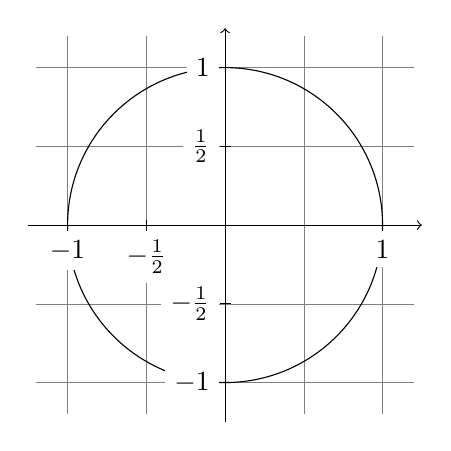
\begin{tikzpicture}[scale=2]
        \draw[step=.5cm, gray, very thin] (-1.2,-1.2) grid (1.2,1.2); 
        \draw[->] (-1.25,0) -- (1.25,0) coordinate (x axis);
        \draw[->] (0,-1.25) -- (0,1.25) coordinate (y axis);
        \draw (0,0) circle (1cm);
        \foreach \x/\xtext in {-1, -0.5/-\frac{1}{2}, 1} 
        \draw (\x cm,1pt) -- (\x cm,-1pt) node[anchor=north,fill=white] {$\xtext$};
        \foreach \y/\ytext in {-1, -0.5/-\frac{1}{2}, 0.5/\frac{1}{2}, 1} 
        \draw (1pt,\y cm) -- (-1pt,\y cm) node[anchor=east,fill=white] {$\ytext$};
      \end{tikzpicture}
      \begin{equation*}
      	[x(t)]^2+[y(t)]^2=r^2
      \end{equation*}
      circonferenza con certro nel origine e raggio r
    \end{multicols}
    Se si ha $\begin{cases} x=x(t) \\ y=y(t) \\ z=z(t)\end{cases}$ al variare di $t\in T \leq R$ si
    ha una curva nello spazio.
\end{esempio}
\begin{esempio}
  $\begin{cases} x = \Gamma \cos t \\ y = \Gamma \sin t \\ z=Kt \end{cases}$ elica circolare 
\end{esempio}
\subsection{Funzione composta}
\begin{defi}
  Sia $\gamma$ la curva $\begin{cases} x=x(t) \\ y=y(t)\end{cases}$ $t\in I < R$
	di codominio B\\
  $I\to B$\\
  Sia f(x,y) definita in A \\
  $t\in f(x(t),y(t))$ se il codominio di $\gamma$ coincide con il codomio di
	$f(x,y)$, cioè
  $B \leq A$
\end{defi}
\subsection{Teorema della derivata della funzione composta}
\begin{defi}
	Sia $\gamma$ la curva di punti $(x(t),y(t))$ e sia derivabile in un
	intervallo $I$ (\underline{cioè esistono })\\
	Sia f(x,y) differenziabile in x(t)\\
	Allora la funzione conposta da $F(t)=f(x(t),y(t))$ è derivabile in I e la
	sua derivata prima vale:
	\begin{equation}
		F^\prime (t)=f_x(x(t),y(t))x^\prime(t)+f_y(x(t),y(t))y^\prime(t)
	\end{equation}
	\begin{equation*}
		\begin{matrix}
			(\nabla f *\Gamma^\prime (t)) & \nabla f \equiv (f_x;f_y) &
			\Gamma^\prime \equiv(x^\prime (t); y^\prime (t))
		\end{matrix}
	\end{equation*}
	\begin{multicols}{2}
		\paragraph{Ipotesi}
			$\gamma \equiv (x(t),y(t))$ derivabile in I\\
			$f(x,y)$ differenziale in x(t)
		\paragraph{Tesi}
		$F(t)=f(x(t),y(t))$ derivabile in I\\
		$F^\prime(t)=f_x(x(t),y(t))x^\prime(t)+f_y(x(t),y(t))y^\prime (t)$
	\end{multicols}
\end{defi}
\begin{proof}
	Devo dimostrare che $\lim\limits_{h\to 0} \frac{F(t+h)-F(t)}{h}=F^\prime
	(t)=F_x(x(t),y(t))x^\prime (t)+f_y(x(t),y(t))y^\prime(t)$\\
	Scrivo l'incremento di F(t) per un h
	\begin{equation*}
		F(t+h)-F(t)=f[x(t+h),y(t+h)]- f[x(t), y(t)] \text{ Per definizione di funzione composta F(t)}
	\end{equation*}
	Poiché f(x,y) è differenziabile si ha 
	\begin{equation*}
		\begin{matrix}
			f[x(t+h),y(t+h)]-f[x(t),y(t)]=f_x\underbrace{[x(t),y(t)]}_{fx}
			\underbrace{[x(t+h)-x(t)]}_h+
			f_y\underbrace{[x(t+h)-y(t+h)]}_{fy}\underbrace{[y(t+h)-y(t)]}_k\\+o
			\left(\sqrt{\underbrace{[x(t+h)-x(t)]^2}_{h^2}
			+  \underbrace{[y(t+h)-y(t)]^2}_{k^2}}\right)
		\end{matrix}
	\end{equation*}
	Divido entrambi i membri per h e calcolo il $\lim_{h\to 0}$
	\paragraph{I membro}
	\begin{equation*}
		\lim_{h\to 0} \frac{f[x(t+h),y(t+h)]-f[x(t),y(t)]}{h}=F^\prime(t)
	\end{equation*}
	\paragraph{II membro}
	\begin{equation*}
		\begin{matrix}
			\lim\limits_{h\to
		0}fx[x(t),y(t)]\underbrace{\left[\frac{x(t+h)-x(t)}{h}\right]}_{x^\prime
		(t)} + \lim\limits_{h\to 0} f_y
		[x(t+h)-y(t+h)]\underbrace{\left[\frac{y(t+h)-y(t)}{h}\right]}_{y^\prime
		(t)}\\ +\lim\limits_{h\to 0}o
			\underbrace{\left(\sqrt{[x(t+h)-x(t)]^2 +
			[y(t+h)-y(t)]^2}\right)}_0
		\end{matrix}
	\end{equation*}
	\begin{equation*}
		F^\prime =f_x[x(t),y(t)]x^\prime(t)+f_y[x(t),y(t)]y^\prime (t)
	\end{equation*}
\end{proof}
\begin{esempio}
	\begin{equation*}
		\begin{matrix}
			z=x^2y & \begin{cases}
				x(t)=-t & F(t)=z(x(t),y(t))=-t^2*t=-t^3\\
				y(t)=t & F^\prime(t)=z^\prime=-3t^2
			\end{cases}
		\end{matrix}
	\end{equation*}
	\begin{equation*}
		F^\prime(t)=f_x(x(t), y(t))x^\prime(t)+f_x(x(t), y(t))y^\prime (t)=z_x
		x^\prime(t)+z_y y^\prime(t) = -3t^2
	\end{equation*}
\end{esempio}
\section{Teorema differenziabilità delle funzioni composite}
\begin{teorema}
	Siano $x=(x_1,x_2,\dots,x_n)$ n funzioni in k variabili
	$t=(t_1,t_2,\dots,t_k)$
	\begin{equation}
		\begin{cases}
			x_1=x_1(t_1,t_2,\dots,t_k)\\
			x_2=x_2(t_1,t_2,\dots,t_k)\\
			\dots\\
			x_n=x_n(t_1,t_2,\dots,t_k)
		\end{cases}
	\end{equation}
	Componiamo le funzioni ottenendo la funzione composita
	\begin{equation*}
		f[x_1(t_1,t_2,\dots,t_k), x_2(t_1,t_2,\dots,t_k), \dots,
		x_n(t_1,t_2,\dots,t_k)]
	\end{equation*}
	Siano ($x_1(t_1,t_2,\dots,t_k), x_2(t_1,t_2,\dots,t_k), \dots,
		x_n(t_1,t_2,\dots,t_k)$) n funzioni definite in un insieme aperto
		$D\leq R^n$ e siano derivabili parzialmente rispetto a $t_i$
		($i=1,2,\dots, k$).\\
		Sia $f(x_1,\dots,x_n)$ una funzione definita in A contenente in
		codominio $x(D)$ e sia f differenziabile in A\\
	Allora la funzione composita $F(t)=x_1(t_1,t_2,\dots,t_k), x_2(t_1,t_2, 
		\dots,t_k), \dots, x_n(t_1,t_2,\dots,t_k)$ è derivabile parzialmente
		rispetto a $t_i(i=1,2,\dots,k)$ nel punto t.
		\begin{equation*}
			\frac{\partial F}{\partial t_i} (t)=\frac{\partial f}{\partial
			x_j}(x(t))+\frac{\partial x_i}{\partial t_i}(t) \text{ (si somma
			sugli inasci ripetuti)}
		\end{equation*}
		Inoltre, se f e ($x_1(t_1,t_2,\dots,t_k), x_2(t_1,t_2,\dots,t_k), \dots,
		x_n(t_1,t_2,\dots,t_k)$) sono di classe $C^1$, anche $F=f(x(t))\in c^1$
		ed è quindi differenziabile.
		\begin{equation*}
			\hbar=k=2 \text{ coordinate polari}
		\end{equation*}
		\begin{equation*}
			\begin{matrix}
				\begin{cases}
					x_1=x\\
					x_2=y
				\end{cases}
				\begin{cases}
					t_1=\varphi\\
					t_2=\varphi
				\end{cases} & f(x,y) &
				\begin{cases}
					x=x(\varphi,\varphi)\\
					y=y(\varphi,\varphi)
				\end{cases}\to \begin{cases}
					x=\rho\cos \varphi\\
					y=\rho \sin \varphi
				\end{cases}
			\end{matrix}
		\end{equation*}
		\begin{equation*}
			f(x,y)=f(\rho\cos\varphi,\rho \sin \varphi)
		\end{equation*}
		\begin{equation*}
			\begin{matrix}
				\frac{\partial f}{\partial \rho}=\frac{\partial f}{\partial x}
				x\rho+\frac{\partial f}{\partial y}y\rho=
				\frac{\partial f}{\partial x} \cos \varphi+
				\frac{\partial f}{\partial y} \sin \varphi\\
				\frac{\partial f}{\partial \rho}=\frac{\partial f}{\partial x}
				x\rho+\frac{\partial f}{\partial y}y\varphi=
				\frac{\partial f}{\partial x} (-\rho\sin \varphi)+
				\frac{\partial f}{\partial y} (\rho\sin \varphi)
			\end{matrix}
		\end{equation*}
\end{teorema}
\section{Differenziale secondo}
\begin{defi}
	$d^2f$ è il differenziale del differenziale primo
        \begin{equation*}
                \begin{matrix}
                        d^2f=d(df)= d(f_xh+f_yk)=\frac{\partial}{\partial x} (f_xh+f_yk)h+ 
                        \frac{\partial}{\partial x}(f_xh+f_yk)k=\\
                        =(f_{xx}h+f_{xy}k)h+ (f_{xy}h+f_{yy}k)k=f_{xx}h^2+f_{xy}k hx+ f_{xy}
                        hx+f_{yy} k^2
                \end{matrix}
         \end{equation*}
         Se $f(x,y)\in c^2$ (derivate parziali II continue) vale il teorema di Schwarz
         (\ref{Schwarz}), cioè $fyx=fxy$ -- Il differenziale secondo allora diventa
         \begin{equation*}
           d^2f=fxxh2+3fxy hk + fyy k^2
         \end{equation*}
         Per ipotesi il gradiente è nulla $\Delta f(x_0,y_0)=0$ cioè $\nabla f(x_0,y_0)\equiv (f_x(x_0,y_0),fy(x_0,y_0))\equiv (0,0)$ ovvero le derivate parziali prime sono nulle
         $fx(x_0,y_0)=0$, $fy(x_0,y_0)=0$ -- Ciò comporta l'annullarsi del differenziale primo
         \begin{equation*}
           df(x_0, y_0)=fx(x_0,y_0)h+fy(x_0,y_0)k=0*h+0*k=0
         \end{equation*}
         Per cui nella foruma di Taylor si ha:
         \begin{equation*}
           f(x,y)=f(x_0,y_0)+\frac{1}{2!}d^2f(x_0+\theta h, y_0+\theta k) \text{ Forme quadratiche}
         \end{equation*}
         Il segno di $f(x,y)-f(x_0,y_0)$ è lo stesso di $\frac{1}{2!}d^2f(x_0+\theta h,
         y_0+\theta k)$, cioè è lo stesso differenziale secondo.\\
         Per ipotesi $det Hp(x_0,y_0)>0$, ($f(x,y)\in C_A^2\Rightarrow$ vale il teorema di Schwarz)
         \begin{equation*}
           \begin{vmatrix}
             fxx(x_0,y_0) & fxy(x_0,y_0) \\
             fyx(x_0,y_0) & fyy(x_0,y_0) 
           \end{vmatrix}= fxx*fyy-fxy^2>0
         \end{equation*}
         e $fxx(x_0,y_0)>0$\\
         Ciò implica per definizione che la forma quadratica associata ad $Hp(x_0,y_0)$ è positiva
         tutto ciò implica $d^2f(x_0+\theta h, y_0+\theta k)>0$\\
         Per cui $f(x,y)-f(x_0,y_0)>0$ 
         \begin{equation*}
           \begin{matrix}
              \text{cioè } f(x,y)>f(x_0,y_0) & \text{ difiniziondi di Minimo relativo (\ref{minmaxrel})}
           \end{matrix}
         \end{equation*}
         quindi $(x_0,y_0)$ è un punto di muinimo relativo\\
         Analogamente, se $f(x_0,y_0)<0$ si dimosta che $(x_0,y_0)$ è un punto di massimo
         relatovo (\ref{minmaxrel})
\end{defi}
\clearpage
\subsection{Condizioni sufficiente per l'esistenza di minimo e massimo relativo}
Sia $f(x,y)$ definita in $A,\text{ } f(x,y)\in C^2_A, \text{ } (x_0,y_0)\in A$\\
Se $\nabla f(x_0,y_0)=0$
\begin{equation*}
  det H_F(x_0,y_0)\begin{cases}
                    >0 \begin{cases}
                         fxx(x_0,y_0)>0 \text{ \color{red} Minimo relativo}\\
                         fxx(x_0,y_0)<0 \text{ \color{red} Massimo relativo}
                       \end{cases}\\
                    <0 \text{ Punto di sella (\underline{non sono presenti Max e min})}\\
                    =0 \text{ Non si vsa se sono presenti Max o min}
                  \end{cases}
\end{equation*}
\begin{esempio}
  Massimi e minimi
  \begin{enumerate}
  \item $z=x^2+y^2$
    \begin{equation*}
      \nabla f=0 \begin{cases}
                   zx=0\\
                   zy=0
                 \end{cases}\begin{cases}
                   2x=0\\
                   -2y=0
                 \end{cases}\begin{cases}
                   x=0\\
                   y=0
                 \end{cases} in (0,0)\text{ }\nabla f=0 \text{ può MAX o MIN}
    \end{equation*}
    \begin{equation*}
		det H_f=\begin{vmatrix}
			z_{xx} & z_{zy} \\
			z_{xy} & z_{yy}
		\end{vmatrix}=\begin{vmatrix}
			2 & 0 \\
			0 & -2
		\end{vmatrix} =-4
    \end{equation*}
    \item Semisuperfici sferica $z=\sqrt{c^2-x^2-y^2}$
		\begin{equation*}
			\nabla f=0 \begin{cases}
				z_x=\frac{-x}{\sqrt{\Gamma^2-x^2-y^2}}\\
				z_y=\frac{-y}{\sqrt{\Gamma^2-x^2-y^2}}
			\end{cases} \text{ dominio D } x^2-y^2<\Gamma^2 
		\end{equation*}
		\begin{equation*}
			\begin{cases}
				z_x=0\\
				z_y=0
			\end{cases}\begin{cases}
					x=0\\
					y=0
			\end{cases} (0,0)\leftarrow D \text{ può esserci un Max e un Min}
		\end{equation*}
		  Verifico e trovo che $det H>0$ $f_{xx}<0: in(0,0)$ è presente il Max.
	  \item Cono $z=\sqrt{x^2+y^2}$ 
		\begin{figure}[ht]
			\centering
			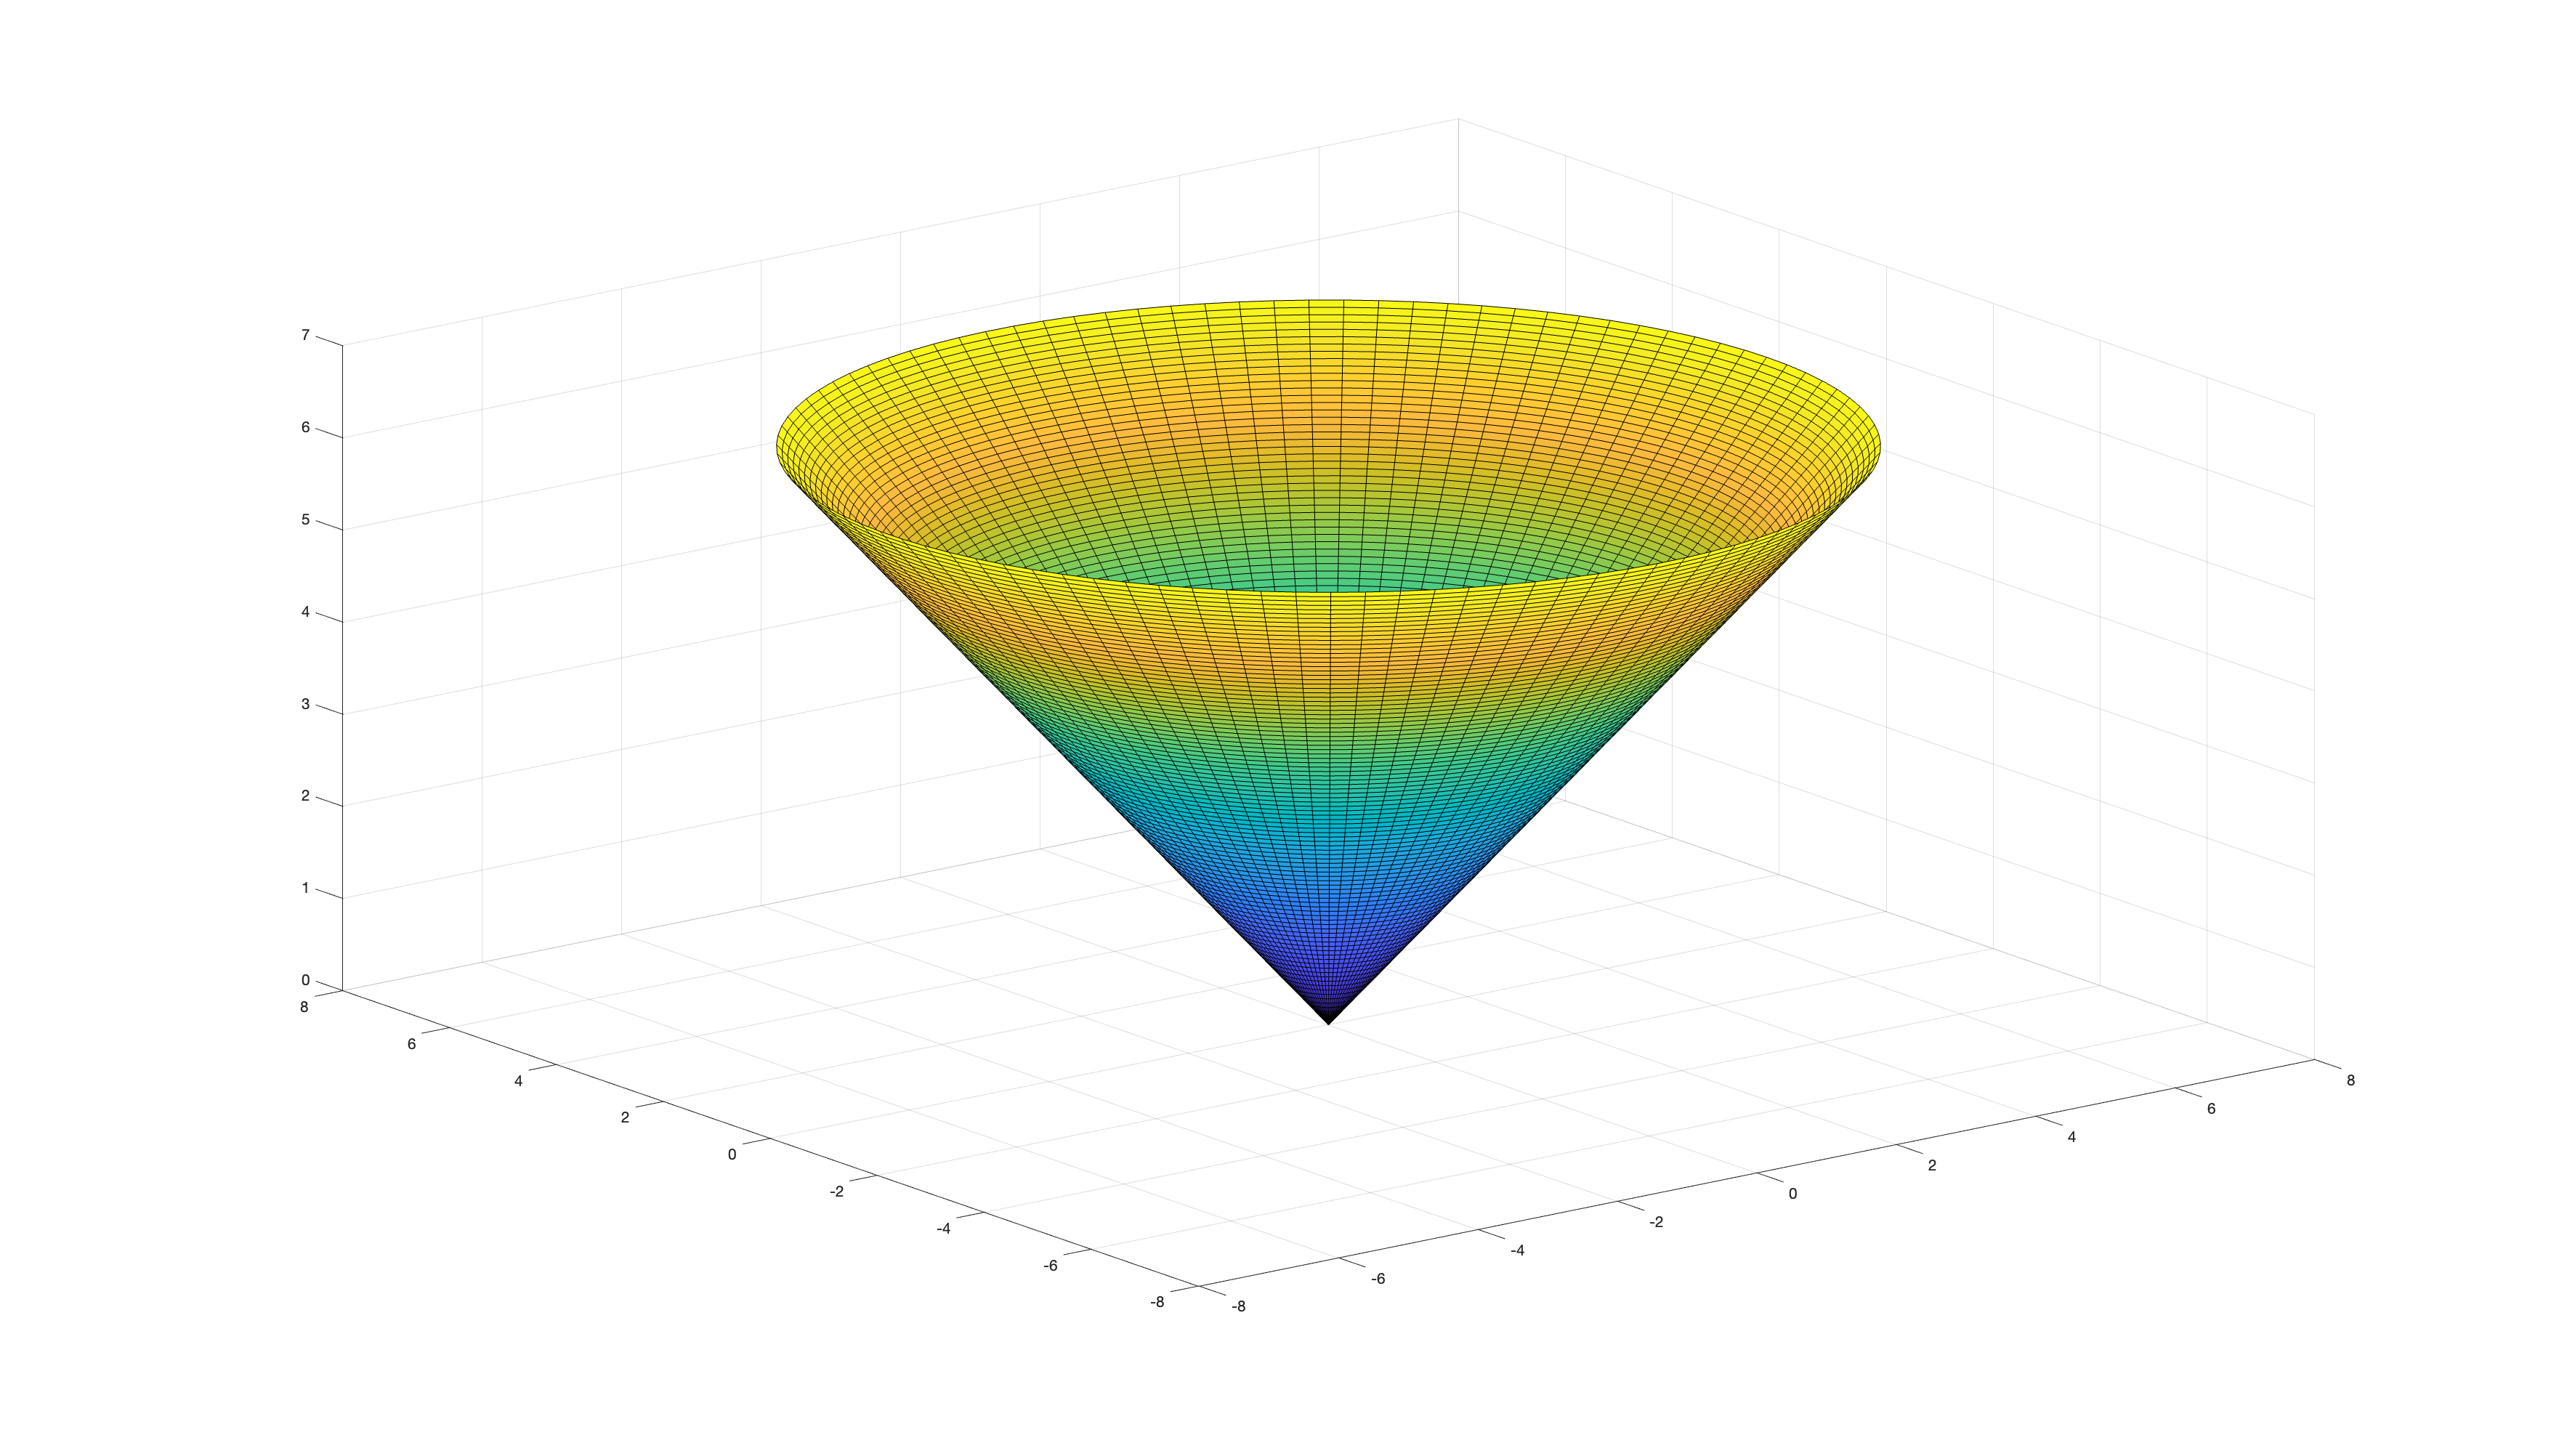
\includegraphics[width=8cm]{img/finiti/cono.eps}
			\caption{Rappresentazione grafica della conica}
			\label{fig:conica}
		\end{figure}
		\begin{equation*}
			\nabla f=0
			\begin{cases}
				z_x=\frac{x}{\sqrt{x^2+y^2}}\\
				z_y=\frac{y}{\sqrt{x^2+y^2}}
			\end{cases}\begin{cases}
					x=0\\
					y=0
			\end{cases} 
		\end{equation*}
		  \begin{nota}
			  sarebbe (0,0) ma il dominio delle derivate $x^2+y^2>0$ cioè
			  $\forall(x,y)\in R^2-\{0,0\}$ in (0,0) non è derivabile.
		  \end{nota}
		  Sappiamo\footnote{si vede geometricamente} che in (0,0) c'è un
		  {\color{red}minimo assoluto}
	  \item $z=x^4 +y^4$
		  \begin{equation*}
			\begin{cases}
				z_x=4x^3=0\\
				z_y=
			\end{cases}\begin{cases}
					x=0\\
					y=0
			\end{cases} \text{ in (0,0) può esserci Max/Min relativo}
		  \end{equation*}
		  \begin{equation*}
			  \begin{matrix}
				det H=\begin{vmatrix}
					0 & 0\\
					0 & 0
				\end{vmatrix} = 0 & \begin{matrix}
					f_{xx}(0,0)=12x^2|_{0,0}=0\\
					f_{xx}(0,0)= 0\\
					f_{yy}(0,0)=12y^2|_{0,0}=0
				  \end{matrix}
			  \end{matrix}
		  \end{equation*}
		  $det H=0 \to$ non so se in (0,0) c'è un massimo o un minimo
		  relativo.\\
		  Per definire se esiste un massimo o un minimo relativo uso:
		  \begin{equation*}
			  \begin{matrix}
				  \min f(x_0,y_0)\leq f(x,y) & 0\leq x^4+y^4 & x^4+y^4\geq 0 &
				  \text{ \underline{SI} $\forall(x,y)$ risulta da
				  $x^4+y^4\geq 0 (0,0)\min$}\\
				  \max f(x_0,y_0)\geq f(x,y) & 0\geq x^4+y^4 & x^4+y^4\leq 0 &
				  \text{ \underline{NO}}
			  \end{matrix}
		  \end{equation*}
  \end{enumerate}
\end{esempio}
\subsection{Ricerca del massimo e del minimo assoluti}
Condizioni sufficienti per l'essistenza del Massimo e del minimo assoluto
\subsubsection{Teorema di Weierstrass}
\begin{teorema}
	Sia f(x,y) definita in D, i continua in D chiuso e limitato, allora il
	minimo e massimo assoluto in D.
	\begin{multicols}{2}
		\paragraph{Ipotesi:}
		\begin{equation*}
			f\in C^0_D
		\end{equation*}
		D chiuso e limitato
		\paragraph{Tesi:}
		$\exists\min$ con $m=f(x_1,y_1), M=f(x_2,y_2)$ tale che $m\leq
		f(x,y)\leq M$
	\end{multicols}
	\paragraph{Ricerca dei punti di Massimo e minimo assoluti:}
	\begin{itemize}
		\item nei punti di massimo o minimo relativo;
		\item nei punti di non derivabilità;
		\item nei punti di frontiera.
	\end{itemize}
	Vanno ricercati quindi nei seguenti modi:
	\begin{enumerate}
		\item $\nabla f=0$ dove il gradiente si annulla;
		\item $\exists \nabla f$ dove il gradiente non esite;
		\item sulla FD sulla frontiera.
	\end{enumerate}
\end{teorema}
\subsubsection{Studio sulla frontiera}
Sia $\xi$ una superficie definita in un insieme D e sia FD la mia frontiera\\
La frontiera FD è una curva\footnote{o insieme di curve} e suoi punti linitano
l'iperbole $\xi$.\\
Possiamo definire la frontiera in forma parametrica
\begin{equation*}
	FD:\begin{cases}
		x=x(t)\\
		y=y(t)
	\end{cases} t\in [a,b] \mathds{R}\to \mathds{R}^2
\end{equation*}
Calcolo la funzione $f(x,y)$ sui punti della frontiera
\begin{equation}
	f(x,y)\to F(t)=f(x(t),y(t))\text{ funzione di 1 variabile}
\end{equation}
studio del massimo e minimo per $F(t)=0\begin{cases}
	F^{\prime\prime}>0 \min\\
	F^{\prime\prime}<0 \max
\end{cases}$\\
Calcolo i valori della funzione nei punti di Massimo/minimo e li confronto con
i valori Massimo/minimo relativi nel dominio e i valori nei punti di non
derivabilità. La frontiera può anche essere in forma cartesiana
\begin{equation}
	\begin{matrix}
		y=y(x) & a\leq x\leq b
	\end{matrix}
\end{equation}
Calcolo la funzione nei punti della frontiera e procedo come visto prima
$f(x,y)\to F(t)=f(x(t),y(t))$
\begin{esempio}
	Determinare il massimo e il mino assoluto di $f(x,y)=
	1+2x^2+\sqrt{x^2+y^2}$ in $D:\{x^2+y^2\leq \Delta\}$
	\begin{enumerate}
		\item $\nabla f=0$
		\item $\nexists \nabla f$
		\item $FD$
	\end{enumerate}
	\begin{enumerate}
		\item $\nabla f(x,y)=0\begin{cases}
				f_x=0\\
				f_y=0
		\end{cases}\begin{cases}
			4x+\frac{x}{\sqrt{x^2+y^2}}\\
			\frac{y}{\sqrt{x^2+y^2}}
		\end{cases}\begin{cases}
			4x+\frac{x}{\abs x}=0\\
			y=0
		\end{cases}$
		\begin{equation*}
			\begin{cases}
				x=0\\
				y=0
			\end{cases}
		\end{equation*}
			$\nabla f=0$ in (0,0) che non è nel C.E. delle derivate parziali
			per cui $\nabla f \neq 0$ $\forall (x,y)\in A$ A dominio $f_x$ e
			$f_y$
		\item $\nexists \nabla f$ le derivate parziali perime sono definite
			$\forall (x,y)\in R^2:x^2+y^2\neq 0$ cioè in $R^2-\{0,0\}$
			\begin{equation*}
				(0,0) \text{ pnto di non derivabilità } f(0,0)=1
			\end{equation*}
		\item FD
			\begin{equation*}
				\begin{matrix}
					D:\{x^2+y^2\leq 4\} & FD: x^2+y^2=4\\
					& \begin{cases}
						x=2\cos t \\
						y=2\sin t
					\end{cases} t\in [0;2\pi]
				\end{matrix}
			\end{equation*}
			Calcolo $f(x,y)$ sui punti di frontiera
			\begin{equation*}
				f(x,y)=F(t)=1+2(2\cos t)^2+\sqrt{(2\cos t)^2+(2\sin t)^2} =
				1+8\cos^2t+2 = 3+8\cos^2t
			\end{equation*}
			Calcolo $F(t)$ agli estremi $t\in[0;2\pi]$ $F(0)=3+8=11$
			$F(2\pi)=3+8=11$\\
			Studio del massimo e del minimo di $F(t)$
			\begin{equation*}
				\begin{matrix}
					F^\prime(t)=0 & 16\cos t(\sin t)=-16\sin t\cos t =0 & t=0&
					t=\pi & t=\frac{\pi}{2}t=\frac{3}{2} \pi
				\end{matrix}
			\end{equation*}
			\begin{equation*}
				F^{\prime\prime}(t)=16(\cos t \cos t -\sin t \sin t) =16(\sin^2
				t- \cos^2 t)
			\end{equation*}
			\begin{equation*}
				\begin{matrix}
					\text{Ottenuti mettendo a F(t) e valori}\\
					\text{dove ci dovrebbero essere un}\\
					\text{massimo e un minimo}
				\end{matrix} \begin{cases}
					F^{\prime\prime}(\pi)=16(-1)=-16<0\text{ }\max\text{ su FD
					}&
					F(\pi) =3+8=11\\
					F^{\prime\prime}(\frac{\pi}{2})=16(-1)=-16>0\text{
					}\min\text{ su
					FD }& F(\frac{\pi}{2}) =3\\
					F^{\prime\prime}(\frac{3\pi}{2})=16(-1)=-16<0\text{
					}\min\text{ su
					FD }& F(\frac{3\pi}{2}) =3
				\end{cases}
			\end{equation*}
	\end{enumerate}
	Ho ottenuto i sequenti valori
	\begin{equation*}
		\begin{matrix}
			1.\text{ }(x,y) \equiv (0,0) & \text{il }\min \text{ è 1 e viene assunto in
			(0,0)} \\
			11.\text{ }t=0,\pi,2\pi & \text{il } \max \text{ è 11 e viene
			assunti in }&
			\begin{cases}
				x=2\cos 0\\
				y=2\sin 0
			\end{cases}\\
			3.\text{ }t=\frac{\pi}{2}, \frac{3}{2}\pi & \begin{cases}
				x=2\cos \pi \\
				y=2\sin \pi
			\end{cases} & (-2,0) & \begin{cases}
				x=2\cos 2\pi \\
				y=2\sin 2\pi
			\end{cases} & (2,0)
		\end{matrix}
	\end{equation*}
\end{esempio}
\subsection{Metodo dei moltiplicatori di di Lagrange}
Nel caso in cui $g(x,y)=0$ non definisca una funzione implicata, per trovare i
massimi e minimi vincolati si introduce una funzione ausiliaria, detta
\underline{\color{red}lagrangiana}, così definita:
\begin{equation}
	F(x,y,\lambda)=f(x,y)+\lambda g(x,y)
\end{equation}
$F(x,y,\lambda)$ è combinazione lineare delle funzioni $f(x,y)$ E $g(x,y)$ --
Il parametro $\lambda$ prende il nome di {\color{red}Moltiplicatore di
Lagrange}. I punti di massimo vincolati sono quelli in cui il gradiente di
$F(x,y,z)$ si annulla ovvero\dots
\begin{equation}
	\nabla F_{(x,y,z)}=0 \begin{cases}
		F_x=fx(x,y)+\lambda g_x(x,y)\\
		F_y=fx(x,y)+\lambda g_y(x,y)\\
		F_\lambda=g(x,y)=0
	\end{cases}
\end{equation}
Si risolve questo sistema di tre equazioni in tre variabili e il valore massimo
della funzione è calcolata nei punti soluzioni è il massimo calcolato e il
valore minimo della funzione calcolata nei punti soluzione è il massimo
vincolato.
